\documentclass[11pt,letterpaper]{article}
%\documentclass[11pt,a4paper]{report}


\usepackage{tikz}
\usepackage{amssymb,amsmath,amsthm} 
\usepackage[margin=2cm]{geometry}
\usepackage{fancyhdr}
\usepackage{enumitem}
\usepackage[compact]{titlesec}
\usepackage{graphicx,ctable,booktabs,subcaption}

\usepackage{xparse,hyperref,parskip}

%\newcommand{\abs}[1]{\left|#1\right|}

\newcommand{\semester}{Spring 2022}
\newcommand{\due}{Thursday, April 14}

\newcommand{\bigo}{\mathcal{O}}

\pagestyle{fancy}
\lhead{ }
\chead{\footnotesize Math 3338\quad  Numerical Methods\quad  \semester}
\rhead{\footnotesize \thepage}
\setlength{\parindent}{0cm}
\setlist{noitemsep}



\newtheorem{theorem}{Theorem}

\input{defs.tex}

%Defines the problem environment with arguments Points and Solution gap
\input{problem_env.tex}





\newcommand{\shrug}[1][]{%
\begin{tikzpicture}[baseline,x=0.8\ht\strutbox,y=0.8\ht\strutbox,line width=0.125ex,#1]
\def\arm{(-2.5,0.95) to (-2,0.95) (-1.9,1) to (-1.5,0) (-1.35,0) to (-0.8,0)};
\draw \arm;
\draw[xscale=-1] \arm;
\def\headpart{(0.6,0) arc[start angle=-40, end angle=40,x radius=0.6,y radius=0.8]};
\draw \headpart;
\draw[xscale=-1] \headpart;
\def\eye{(-0.075,0.15) .. controls (0.02,0) .. (0.075,-0.15)};
\draw[shift={(-0.3,0.8)}] \eye;
\draw[shift={(0,0.85)}] \eye;
% draw mouth
\draw (-0.1,0.2) to [out=15,in=-100] (0.4,0.95); 
\end{tikzpicture}}

\begin{document}

\begin{center}
{\huge{\bf  Numerical Methods}} \\[1.5ex]
{\bf Math 3338 -- \semester}\\[1.5ex]
{\Large{\bf Worksheet 24\ \\[2ex] Fourier Transforms}}\\
\end{center}
\vspace{2mm}


\section{Reading}

\begin{table}[!ht]
 \centering
 \begin{tabular}{lc}
   CP &  7.1, 7.3 \\
 NMEP &  -
 \end{tabular}
\caption{Sections Covered}
\end{table}

\section{Complex Fourier Transform}
There are many ways to represent a function. Perhaps the most useful is a series expansion,
\[
 f(x) = \sum \gamma_k g_k(x)
\]
where the $g_k(x)$'s are ``nice'' in some way. Naturally this raises the question, what are the
$\gamma_k$'s and how do we find them?

If we choose the $g_k$'s correctly, we'll have 
\[
 \gamma_k = \int_a^b f(x) \bar{g}_k(x)\,dx
\]
where $\bar{g}_k(x)$ is the complex conjugate of $g_k(x)$. This is a natural consequence of the
$g_k(x)$'s forming an orthonormal basis of the space of functions. That's not really important right
now, but it is in life.

Suppose our interval is $[a,b]$, set $L=b-a$ the width of the interval. Then the complex
Fourier transform is given by\footnote{Typically the $\frac{1}{\sqrt{L}}$ is not included here but
there is a $\frac{1}{L}$ later. This is all fine. But MATH wants it there. We'll drop it for 
good reason later though.},
\[
 g_k(x) = \frac{1}{\sqrt{L}} e^{k\frac{2\pi ix}{L}}
\]
Then we'll be able to write $f(x)$ as,
\[
 f(x) = \sum_{k=-\infty}^\infty \gamma_k g_k(x)
\]
Of course, an infinite number of coefficients may not be ideal from a computational point of view.
So we restrict to be
\[
 f(x) = \sum_{k=-N}^N \gamma_k g_k(x)
\]
Where $N$ is an integer. You do want this to be symmetric if $f(x)$ is a real valued function.

The $k$'s are frequencies and the $\gamma_k$ is the amplitude at the given frequency.



\section{Real Fourier Transform}

Most functions we deal with are real valued functions. Using the complex Fourier transform is a 
bit of overkill, so we'd like a real version. This exists. But keeping it real does occasionally
lead to issues\footnote{\url{https://www.youtube.com/watch?v=pfz0tDQZhqs}.}


As we all know, $e^{ix} = \cos(x) + i\sin(x)$. This is essentially the idea to get the real Fourier
transform. In fact, there are two. The cosine transform,
\[
 c_k(x) = \frac{1}{L}\cos\left(2k\pi x\right)
\]
and the sine transform,
\[
 s_k(x) = \frac{1}{L} \sin\left(2k\pi x\right)
\]

However, since cosine is an even function and function we use the cosine transform must be 
symmetric about the midpoint of the interval. Similarly, since sine is odd the function must 
be anti-symmetric about the midpoint. Luckily, these issues are not difficult to overcome, you just
double the interval and modify the function. Figure \ref{fig:even} shows $f(x)=x$ on $[0,2]$. 
\begin{figure}[!ht]
 \centering
 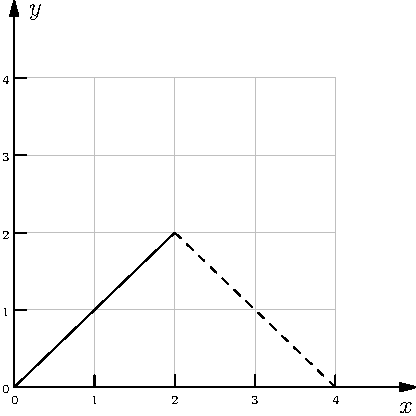
\includegraphics{images/even.pdf}
 \caption{The solid line of $f(x)$, the dashed line gets included for the cosine transform}
 \label{fig:even}
\end{figure}
For the cosine transform to work properly, we need to include the dashed line as well.













\newpage

\begin{center}
{\huge{\bf  Numerical Methods}} \\[1.5ex]
{\bf Math 3338 -- \semester}\\[1.5ex]
{\Large{\bf Homework 24 (Due: \due)}}\\
\end{center}
\vspace{2mm}

Include all graphs in your write up of the problems.


\begin{problem}
Write two functions \texttt{complex\_fourier} and \texttt{inverse\_complex\_fourier}. Use
the trapezoid method with 1000 subintervals for your integration technique.

For \texttt{complex\_fourier} the inputs should be a function $f$, $a$, $b$ and $N$. Return a
$(2N+1)\times 2$ array where the first column is the frequency $k$, and the second column is $\gamma_k$.


For \texttt{inverse\_complex\_fourier} the inputs should be the array returned by the previous function,
$x$, $a$, and $b$. It should return a number.
\end{problem}


\begin{problem}
 Let $f(x) = x$ on the interval $[-1,1]$. Make a plot of $f(x)$ and the inverse fourier transform of 
$f(x)$ on the same plot for the following situations (make a plot for each situation).
\begin{enumerate}
 \item $N=10$
 \item $N=50$
 \item $N=100$
\end{enumerate}
Describe what you see in each plot. Why do you think the graph looks so funky at the ends of the
interval?

\end{problem}


\begin{problem}
 Let $f(x) = 1-x^2$ on the interval $[-1,1]$. Compute the Fourier transform of $f(x)$ using $N=50$.
\begin{enumerate}
 \item Make a plot of $f(x)$ and the inverse Fourier transform on the same plot. What happened here?
 \item Make a plot of the inverse Fourier transform on the interval $[-5,5]$. Why did this happen?
 \item Make a plot of amplitude vs frequency for the Fourier transform. Be sure to take the absolute
value of the amplitudes as the values are complex. This graphs shows you which frequencies are 
contributing the most to the graph. What is a rough range where the frequencies are ``important''?
\end{enumerate}
\end{problem}



\begin{problem}
 Write two functions \texttt{real\_fourier} and \texttt{inverse\_real\_fourier}. Use the cosine
transform and the trapezoid method with 1000 subintervals for your integration technique. This transformation
will only work for intervals of the form $[a,b]$ with $a,b\ge 0$.


For \texttt{real\_fourier} the inputs should be a function $f$, $a$, $b$ and $N$. Return a
$(N+1)\times 2$ array where the first column is the frequency $k$, and the second column is $\gamma_k$.
There is one detail, for the $k=0$ frequency, you need to divide the amplitude by 2, but only for
that frequency\footnote{There is a reason for this. Try to figure it out.} \footnote{At the end of the
day, it was the real fourier transform that was complex.}. 

For \texttt{inverse\_real\_fourier} the inputs should be the array returned by the previous function,
$x$, $a$, and $b$. It should return a number. For the inverse \textit{you do not need the $\frac{1}{L}$
factor}.
\end{problem}



\begin{problem}
 Let $f(x) = \cos(6\pi x) + 2\cos(8\pi x) - 3\cos(10\pi x)$ on the interval $[0,1]$. Let $N=50$.
\begin{enumerate}
 \item Make a plot of $f(x)$ and the real inverse Fourier transform on the same plot.
 \item Make a plot of amplitude vs frequency for the Fourier transform (you don't need the absolute
value). What do you see? Why did this happen?
 \item Do the above two again on the interval $[0,2]$. Does anything change? 
\end{enumerate}
\end{problem}

\newpage

\begin{problem}
 Let $f(x) = \cos(6\pi x) + 2\cos(8\pi x) - 3\cos(10\pi x)$ on the interval $[0,b]$. In this 
problem you'll be making plots of amplitude vs frequency for various values of $b$. Let $N=50$.
\begin{enumerate}
 \item $b=1$
 \item $b=5$
 \item $b=10$
 \item $b=20$
\end{enumerate}
Explain what you see and why you think it is happening.
\end{problem}



\end{document}








































